%%%%%%%%%%%%%%%%%%%%%%%%%%%%%%%%%%%%%%%%%
% Programming/Coding Assignment
% LaTeX Template
%
% This template has been downloaded from:
% http://www.latextemplates.com
%
% Original author:
% Ted Pavlic (http://www.tedpavlic.com)
%
% Note:
% The \lipsum[#] commands throughoutfig.1. this template generate dummy text
% to fill the template out. These commands should all be removed when
% writing assignment content.
%
% This template uses a Perl script as an example snippet of code, most other
% languages are also usable. Configure them in the "CODE INCLUSION
% CONFIGURATION" section.
%
%%%%%%%%%%%%%%%%%%%%%%%%%%%%%%%%%%%%%%%%%

%----------------------------------------------------------------------------------------
%	PACKAGES AND OTHER DOCUMENT CONFIGURATIONS
%----------------------------------------------------------------------------------------

\documentclass{article}

\usepackage{fancyhdr} % Required for custom headers
\usepackage{lastpage} % Required to determine the last page for the footer
\usepackage{extramarks} % Required for headers and footers
\usepackage[usenames,dvipsnames]{color} % Required for custom colors
\usepackage{graphicx} % Required to insert images
\usepackage{listings} % Required for insertion of code
\usepackage{courier} % Required for the courier font
\usepackage{lipsum} % Used for inserting dummy 'Lorem ipsum' text into the template
\usepackage[utf8]{inputenc}
\usepackage{amsmath,amssymb,amsfonts,amsthm,graphicx,enumitem}
\usepackage[parfill]{parskip}
\usepackage{color}
\usepackage{float}
\usepackage[ruled,vlined]{algorithm2e}
% Margins
\topmargin=-0.45in
\evensidemargin=0in
\oddsidemargin=0in
\textwidth=6.5in
\textheight=9.0in
\headsep=0.25in

\linespread{1.1} % Line spacing

% Set up the header and footer
\pagestyle{fancy}
\lhead{\hmwkAuthorName} % Top left header
\chead{\hmwkClass\ (\hmwkClassInstructor\ \hmwkClassTime): \hmwkTitle} % Top center head
\rhead{\firstxmark} % Top right header
\lfoot{\lastxmark} % Bottom left footer
\cfoot{} % Bottom center footer
\rfoot{Page\ \thepage\ of\ \protect\pageref{LastPage}} % Bottom right footer
\renewcommand\headrulewidth{0.4pt} % Size of the header rule
\renewcommand\footrulewidth{0.4pt} % Size of the footer rule

\setlength\parindent{0pt} % Removes all indentation from paragraphs

%----------------------------------------------------------------------------------------
%	CODE INCLUSION CONFIGURATION
%----------------------------------------------------------------------------------------

\definecolor{MyDarkGreen}{rgb}{0.0,0.4,0.0} % This is the color used for comments
\lstloadlanguages{Perl} % Load Perl syntax for listings, for a list of other languages supported see: ftp://ftp.tex.ac.uk/tex-archive/macros/latex/contrib/listings/listings.pdf
\lstset{language=Perl, % Use Perl in this example
        frame=single, % Single frame around code
        basicstyle=\small\ttfamily, % Use small true type font
        keywordstyle=[1]\color{Blue}\bf, % Perl functions bold and blue
        keywordstyle=[2]\color{Purple}, % Perl function arguments purple
        keywordstyle=[3]\color{Blue}\underbar, % Custom functions underlined and blue
        identifierstyle=, % Nothing special about identifiers
        commentstyle=\usefont{T1}{pcr}{m}{sl}\color{MyDarkGreen}\small, % Comments small dark green courier font
        stringstyle=\color{Purple}, % Strings are purple
        showstringspaces=false, % Don't put marks in string spaces
        tabsize=5, % 5 spaces per tab
        %
        % Put standard Perl functions not included in the default language here
        morekeywords={rand},
        %
        % Put Perl function parameters here
        morekeywords=[2]{on, off, interp},
        %
        % Put user defined functions here
        morekeywords=[3]{test},
       	%
        morecomment=[l][\color{Blue}]{...}, % Line continuation (...) like blue comment
        numbers=left, % Line numbers on left
        firstnumber=1, % Line numbers start with line 1
        numberstyle=\tiny\color{Blue}, % Line numbers are blue and small
        stepnumber=5 % Line numbers go in steps of 5
}

% Creates a new command to include a perl script, the first parameter is the filename of the script (without .pl), the second parameter is the caption
\newcommand{\perlscript}[2]{
\begin{itemize}
\item[]\lstinputlisting[caption=#2,label=#1]{#1.pl}
\end{itemize}
}

%----------------------------------------------------------------------------------------
%	DOCUMENT STRUCTURE COMMANDS
%	Skip this unless you know what you're doing
%----------------------------------------------------------------------------------------

% Header and footer for when a page split occurs within a problem environment
\newcommand{\enterProblemHeader}[1]{
\nobreak\extramarks{#1}{#1 continued on next page\ldots}\nobreak
\nobreak\extramarks{#1 (continued)}{#1 continued on next page\ldots}\nobreak
}

% Header and footer for when a page split occurs between problem environments
\newcommand{\exitProblemHeader}[1]{
\nobreak\extramarks{#1 (continued)}{#1 continued on next page\ldots}\nobreak
\nobreak\extramarks{#1}{}\nobreak
}

\setcounter{secnumdepth}{0} % Removes default section numbers
\newcounter{homeworkProblemCounter} % Creates a counter to keep track of the number of problems

\newcommand{\homeworkProblemName}{}
\newenvironment{homeworkProblem}[1][Problem \arabic{homeworkProblemCounter}]{ % Makes a new environment called homeworkProblem which takes 1 argument (custom name) but the default is "Problem #"
\stepcounter{homeworkProblemCounter} % Increase counter for number of problems
\renewcommand{\homeworkProblemName}{#1} % Assign \homeworkProblemName the name of the problem
\section{\homeworkProblemName} % Make a section in the document with the custom problem count
\enterProblemHeader{\homeworkProblemName} % Header and footer within the environment
}{
\exitProblemHeader{\homeworkProblemName} % Header and footer after the environment
}

\newcommand{\problemAnswer}[1]{ % Defines the problem answer command with the content as the only argument
\noindent\framebox[\columnwidth][c]{\begin{minipage}{0.98\columnwidth}#1\end{minipage}} % Makes the box around the problem answer and puts the content inside
}

\newcommand{\homeworkSectionName}{}
\newenvironment{homeworkSection}[1]{ % New environment for sections within homework problems, takes 1 argument - the name of the section
\renewcommand{\homeworkSectionName}{#1} % Assign \homeworkSectionName to the name of the section from the environment argument
\subsection{\homeworkSectionName} % Make a subsection with the custom name of the subsection
\enterProblemHeader{\homeworkProblemName\ [\homeworkSectionName]} % Header and footer within the environment
}{
\enterProblemHeader{\homeworkProblemName} % Header and footer after the environment
}

%----------------------------------------------------------------------------------------
%	NAME AND CLASS SECTION
%----------------------------------------------------------------------------------------

\newcommand{\hmwkTitle}{Machine learning methods for stock return series analysis via python} % Assignment title
\newcommand{\hmwkDueDate}{2015/05/03} % Due date
\newcommand{\hmwkClass}{Python final project report} % Course/class
\newcommand{\hmwkClassTime}{3:30PM} % Class/lecture time
\newcommand{\hmwkClassInstructor}{Instructor:Dr.Jinfeng Zhang} % Teacher/lecturer
\newcommand{\hmwkAuthorName}{Jian Wang } % Your name

%----------------------------------------------------------------------------------------
%	TITLE PAGE
%----------------------------------------------------------------------------------------

\title{
\vspace{2in}
\textmd{\textbf{\hmwkClass:\ \hmwkTitle}}\\
\normalsize\vspace{0.1in}\small{Due\ on\ \hmwkDueDate}\\
\vspace{0.1in}\large{\textit{\hmwkClassInstructor\ \hmwkClassTime}}
\vspace{3in}
}

\author{\textbf{\hmwkAuthorName}}
\date{} % Insert date here if you want it to appear below your name

%----------------------------------------------------------------------------------------

\begin{document}

\maketitle

%----------------------------------------------------------------------------------------
%	TABLE OF CONTENTS
%----------------------------------------------------------------------------------------

%\setcounter{tocdepth}{1} % Uncomment this line if you don't want subsections listed in the ToC

\newpage
\tableofcontents
\newpage

%% insert the programming code
%\begin{homeworkProblem}
%Listing \ref{homework_example} shows a Perl script.
%
%\perlscript{homework_example}{Sample Perl Script With Highlighting}
%
%\lipsum[1]
%\end{homeworkProblem}

%% insert the chart
%\begin{homeworkProblem}
%\lipsum[2]
%
%\problemAnswer{
%\begin{center}
%\includegraphics[width=0.75\columnwidth]{example_figure} % Example image
%\end{center}
%\lipsum[3-5]
%}
%\end{homeworkProblem}
%% Example of list array and emurate
%\begin{homeworkProblem}
%
%\begin{flalign}
%A =
%\begin{bmatrix}
%A_{11} & A_{21} \\
%A_{21} & A_{22}
%\end{bmatrix}
%\end{flalign}
%
%\begin{itemize}
%	\item First item in a list
%		\begin{itemize}
%		\item First item in a list
%			\begin{itemize}
%			\item First item in a list
%			\item Second item in a list
%			\end{itemize}
%		\item Second item in a list
%		\end{itemize}
%	\item Second item in a list
%\end{itemize}
%
%\begin{enumerate}
%\item First item in a list
%\item Second item in a list
%\item Third item in a list
%\end{enumerate}

%% equation formula
%$\left \{
%\begin{tabular}{l}
%$V_t+\frac{\sigma^2S^2}{2}V_{SS}+rSV_s - rV=0$\\
%
%$V(0,t)=e^{-r(T-t)}$\\
%
%$V(\infty,t)=0$\\
%
%$V(S,T)=I_{\{S\leq K\}}$
%\end{tabular}
%\right.$

%\end{homeworkProblem}
%----------------------------------------------------------------------------------------

\begin{homeworkProblem}

\section*{[Summary]}
1) Python consumed less CPU time than R for Logistic, Ridge, Lasso regression and support vector machine methods.\\

2) lasso ($\lambda$=0.01) and svm (rbf) performed good for both two languages.\\

3)Python performed better in most cases but the difference between the two languages was not
significant.\\

4) For the same day return series analysis, the results were fairly good, however, for the prediction models, the results were close to random guess.\\

5) May reflected the efficient market theorem and can use the high frequency data to see if the results for prediction can be improved.\\

\section{[Introduction]}
\begin{itemize}
\item \textbf{Machine Learning:} Machine learning is a method of teaching computers to make predictions based on historical data.  It is one important branch of artificial intelligence research area. Nowadays, those popular algorithms have been widely used in our financial engineering research area, for example, prediction of stock trend,  deal with big data problem such as limit order book problem.
\item \textbf{Goal:} In our research, we try to deal with the following tasks: \textbf{First}, combine Bayesian network and graphical lasso algorithm to deal with the high dimensional problem. \textbf{Second}, compare the efficiency of machine learning packages of language R and python. \textbf{Finally}, use machine learning methods to deal with the real world stock return data and try to predict the stock return series via those machine learning methods.  \\
\end{itemize}

\section{[Dataset]}
The dataset is named stockdata which from huge package in R. It contained data that were
originally obtained from Yahoo! Finance. There are 1,258
observations representing 1,258 sequential trading days(form Jan 1 2003 to Jan 1 2008) and 452
variables, each of which was the day's closing price for a different
stock within the Standard \& Poor's 500.We also added two index into the data set, one is S\&P 500 and another is Nasdaq(so totally 454 variables).\\
Among all the stock data , we used Goldman Sachs stock return
series as our response variable and other stocks as the predictors to analyze the stock return series movement.

\newpage

\textbf{Company and price:}:\\
\begin{figure}[H]\centering
  \begin{center}
    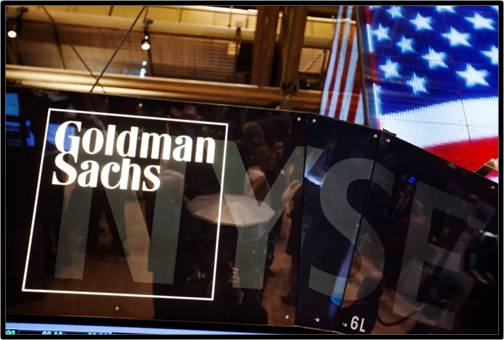
\includegraphics[width=0.5\textwidth, height=0.25\textheight]{gschart.jpg}
      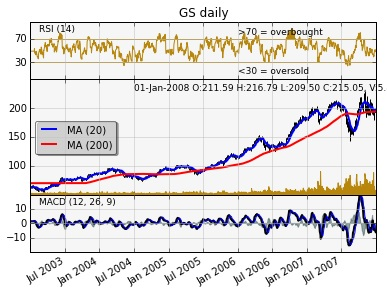
\includegraphics[width=0.5\textwidth, height=0.25\textheight]{gs_plot.jpg}
  \end{center}
\caption{Goldman Sachs Company and prices}\label{fig.1.}
\end{figure}


\section{[Methodology]}

\textbf{1.Bayesian network}\\
BN(Bayesian network) is a probabilistic graphical model (a type of statistical model)
that represents a set of random variables and their conditional dependencies via a directed acyclic graph (DAG)\\
The following chart is an example of BN:\\
\begin{figure}[H]
  \begin{center}
    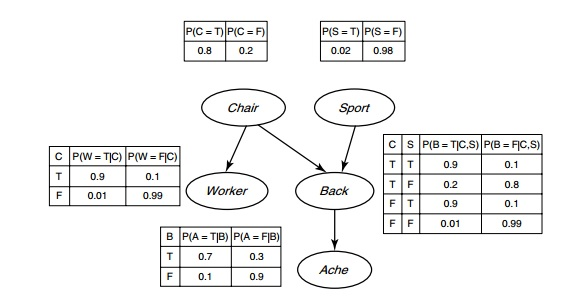
\includegraphics[width=0.5\textwidth, height=0.3\textheight]{bayesian.jpg}\\
  \end{center}
\caption{Bayesian networks example}\label{fig.2.}
\end{figure}

Our main concern is on the structure learning process since the structure learning process is exponentially increasing complicated and is the most challenging part in Bayesian network research area. The standard that we used to choose the optimal structure is the score based method.\\
\vspace{2ex}
BIC score:$BIC=-2*ln\hat{L}+K*ln(n)$, where:\\
\vspace{2ex}
$\hat{L}=$ maximum likelihood estimator, $k$ is the number of free parameters and $n$ is the number of observations, ie, the sample size.\\

\textbf{2.Regression models}\\
1) Linear regression:\\
\begin{equation}
\hat{\beta}^{ls}=argmin_{\beta}\{\sum_{i=1}^p{(y_i-\hat{y_i})^2}\}
\end{equation}
2) Logistic Regression
\begin{equation}
ln{\frac{F(x)}{1-F(x)}}=\beta_0+\sum_i\beta_ix_i
\end{equation}

3) Ridge regression:\\
\begin{equation}
\hat{\beta}^{ridge}=argmin_{\beta}\{\sum_{i=1}^p{(y_i-\hat{y_i})^2}+{\color{red}\lambda \sum_{j=1}^p\beta_j^2}\}
\end{equation}

\textbf{Coefficients and paths:}\\

\begin{figure}[H]\centering

     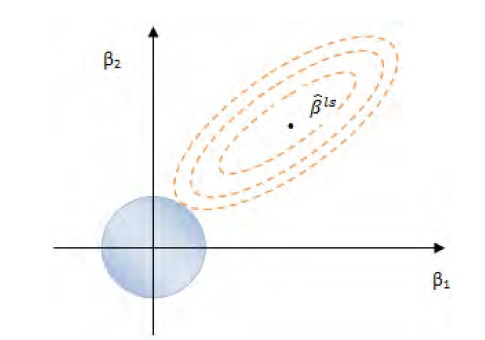
\includegraphics[width=0.3\textwidth, height=0.2\textheight]{ridge.jpg}
     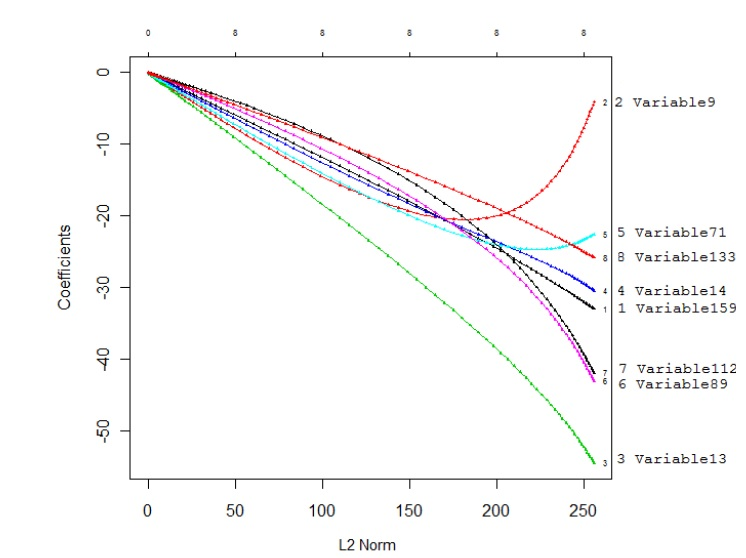
\includegraphics[width=0.3\textwidth, height=0.2\textheight]{ridge_p.jpg}
\caption{Ridge regression coefficients and Paths} \label{fig.3.}
\end{figure}

4) Lasso regression:\\
\begin{equation}
\hat{\beta}^{lasso}=argmin_{\beta}\{\sum_{i=1}^p{(y_i-\hat{y_i})^2}+{\color{red}\lambda\sum_{j=1}^p |\beta_j|}\}
\end{equation}

\textbf{Coefficients and paths}:
\begin{figure}[H]\centering
  \begin{center}
     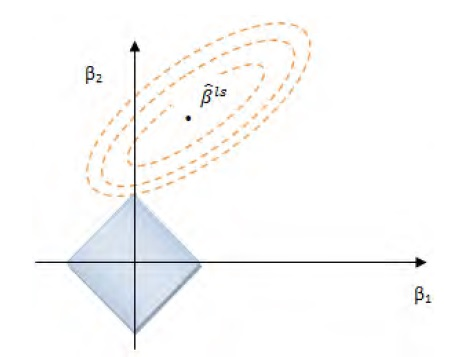
\includegraphics[width=0.3\textwidth, height=0.2\textheight]{lasso.jpg}
     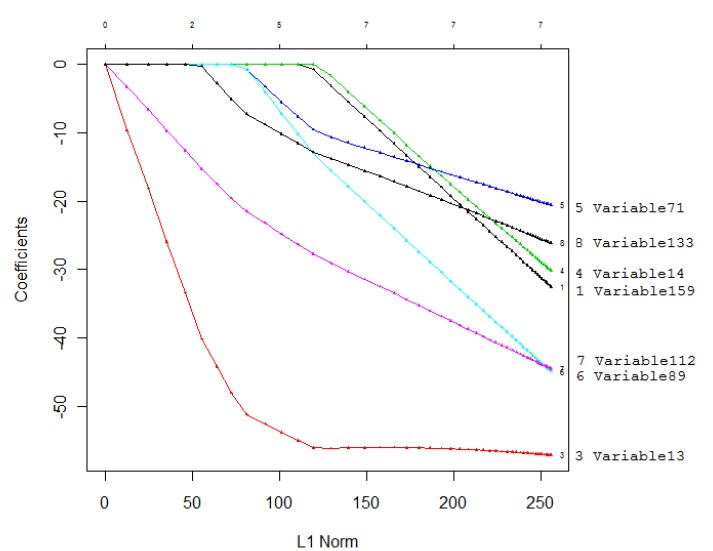
\includegraphics[width=0.3\textwidth, height=0.2\textheight]{lasso_p.jpg}
  \end{center}
\caption{Lasso regression coefficients and paths } \label{fig.4.}
\end{figure}



\textbf{3.Combined models}\\
1) Graphical lasso:
    Suppose we have N multivariate normal observations of dimension p , with mean $\mu$ and covariacne $\Sigma$. Let $\Theta=\Sigma^{-1}$ and $S$ be the empirical covariance matrix, the problem is to maximize the log- likelihood \\
    \begin{center}
    $lnP(X|u,\Sigma)=-\frac{N}{2}ln|\Sigma|-\frac{1}{2}\sum(x_n-u)^T \Sigma^{-1}(x_n-u)$\\
    combined with the $L_1$ penalty\\
    $ln |\Theta|- tr(S\Theta))-\lambda||\Theta||_1$
  \end{center}

Algorithm:\\
  Many algorithms for this problem, The following might be the oldest and simple one by Meinshausen and Buhlmann(2006)problem
    \begin{itemize}
        \item  Estimate a sparse graphical model by fitting a lasso model to each variable, using others as predictors
        \item  Set $\Sigma_{ij}^{-1}$ to be non zero, if either the estimated coefficient of variable i on j, or the
        estimated coefficient of variable j on i, is non-zero
    \end{itemize}

2)  {Bayesian-Glasso model}\\
 For the high dimensional problem, it is not very easy to built the Bayesian network due to its exponentially increasing complexity. \\
 Our idea is to first use the Glasso model to conduct the model selection and then use Bayesian network structure learning process
 to define the network structure. \\
Algorithm:\\
    \begin{itemize}
        \item  Use Glasso algorithm to find the edges among variables
        \item  Use greedy search methods to change the direction only on those existed edges
        \item  Choose the direction which has the optimal BIC score
        \item  Finish when all the edges are reached or attain the maximum iteration numbers
    \end{itemize}

3) Support vector machine\\
\begin{figure}[H]
  \begin{center}
     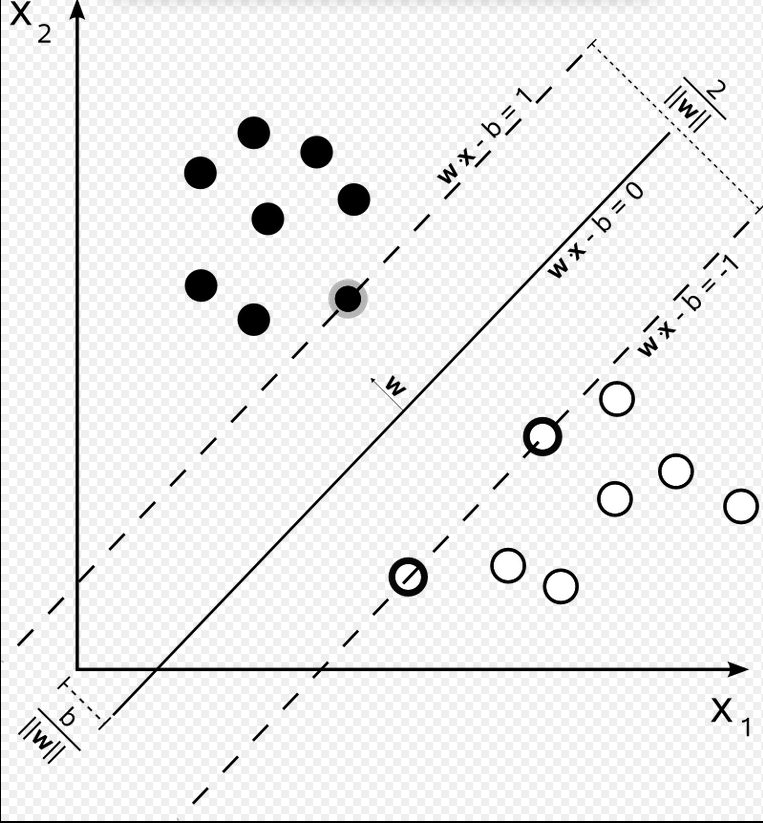
\includegraphics[width=0.3\textwidth, height=0.2\textheight]{svm.png}
  \end{center}
\caption{Support vector machine} \label{fig.5.}
\end{figure}

Try to maximize the margin: $r=1/||w||,y_j=1,-1$\\

Primal form:\\
$\max\limits_{W,b}\ r= 1/||W||$\\
$s.t.(W^Tx_j+b)y_j>=1$\\

Dual form:\\
$\max\limits_{\alpha_1,...,\alpha_M}\ \sum\alpha_l-\frac{1}{2}\sum_{j=1}^{M}\sum_{k=1}^{M}\alpha_j\alpha_k y_j y_k<X_j,X_k>$\\
s.t.$\alpha_l\geq 0$, $\sum_{l=1}^{M}\alpha_ly_l=0$\\

The SVM was trying to deal with high dimensional problems:\\
Sometimes, in lower dimension we can not separate the data properly, so we need to project the data to the high dimensions.\\
Examples:\\
\begin{figure}[H]\centering
  \begin{center}
     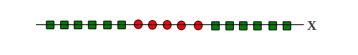
\includegraphics[width=0.3\textwidth, height=0.2\textheight]{1d.png}
     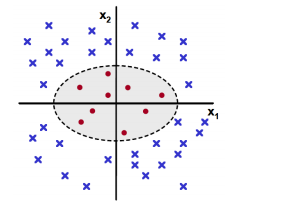
\includegraphics[width=0.3\textwidth, height=0.2\textheight]{2d.png}
  \end{center}
\caption{1d to 2d example} \label{fig.6.}
\end{figure}


\begin{figure}[H]
  \begin{center}
     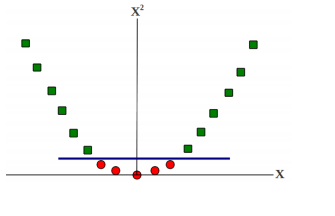
\includegraphics[width=0.3\textwidth, height=0.2\textheight]{1d_2.png}
     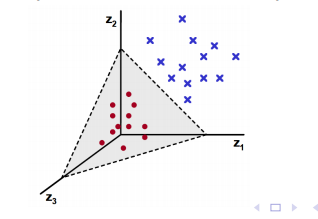
\includegraphics[width=0.3\textwidth, height=0.2\textheight]{2d_2.png}
  \end{center}
\caption{2d to 3d example} \label{fig.7.}
\end{figure}

Kernel functions\\
We can use the kernel function to calculate the inner product in high dimensional cases in its original feature spaces.
{Example:\\}
$k(x,z)=(x^Tz)^2$\\
$=(x_1z_1+x_2z_2)^2$\\
$=x_1^2z_1^2+x_2^2 z_2^2+2x_1x_2z_1z_2$\\
$=(x_1^2,\sqrt{2}x_1x_2,x_2^2)^T(z_1^2,\sqrt{2}z_1z_2,z_2^2)$\\
$=\Phi(x)^T\Phi(z)$\\

\textbf{Kernel functions that we used:}
\begin{itemize}
        \item  Linear kernel\\
        \item  Polynomial Kernel\\
        \item  Radial basis function kernel\\
    \end{itemize}



\section{[Numerical results]}

\begin{itemize}
        \item  Same day stock return series analysis:\\
        we use the same day stock return series to build the machine learning models. For the Bayesian network, we only use the R package. For the  logistic regression, ridge regression, lasso and svm, we used different languages(R and Python) and also compare the CPU time.
        To test the accuracy rate of model, we choose the first 1000 data as training data and the last remaining 257 data as testing. GS as response(discretized as 1 and -1) and the other 453 stocks as predictors.\\
        \item  Predict the stock data:\\
        we used the last one day, two day,... to last five day stock returns as the predictors and today's GS return series as response to see if our model can be used to predict the stockdata.\\
        Still use the first 1000 data as training and the remaining 252 data as testing. GS as the response and the other 2270 variables as predictors.\\
    \end{itemize}


\textbf{1. For the same day return series analysis:}\\
Simple example for Bayesian networks, we chose 10 different world class company from 5 industries, 2 companies from each.\\
 \begin{table}[h!]
  \caption{10 companies}
\begin{center}
    \begin{tabular}{| c | c| c | }
    \hline
    Stock code& Industry & Company name\\
    \hline
GS&Financials&Goldman Sachs Group\\
JPM&Financials&JPMorgan Chase \& Co.\\
MSFT&Information Technology&Microsoft Corp.\\
IBM&Information Technology&International Bus. Machines\\
T&Telecommunications Services&AT\&T Inc\\
VZ&Telecommunications Services&Verizon Communications\\
WMT&Consumer Staples&Wal-Mart Stores\\
KO&Consumer Staples&Coca Cola Co.\\
AMZN&Consumer Discretionary&Amazon.com Inc\\
BBY&Consumer Discretionary&Best Buy Co. Inc.\\

\hline
\end{tabular}
\end{center}
\end{table}

Results for simple cases:\\
\begin{figure}[H]\centering
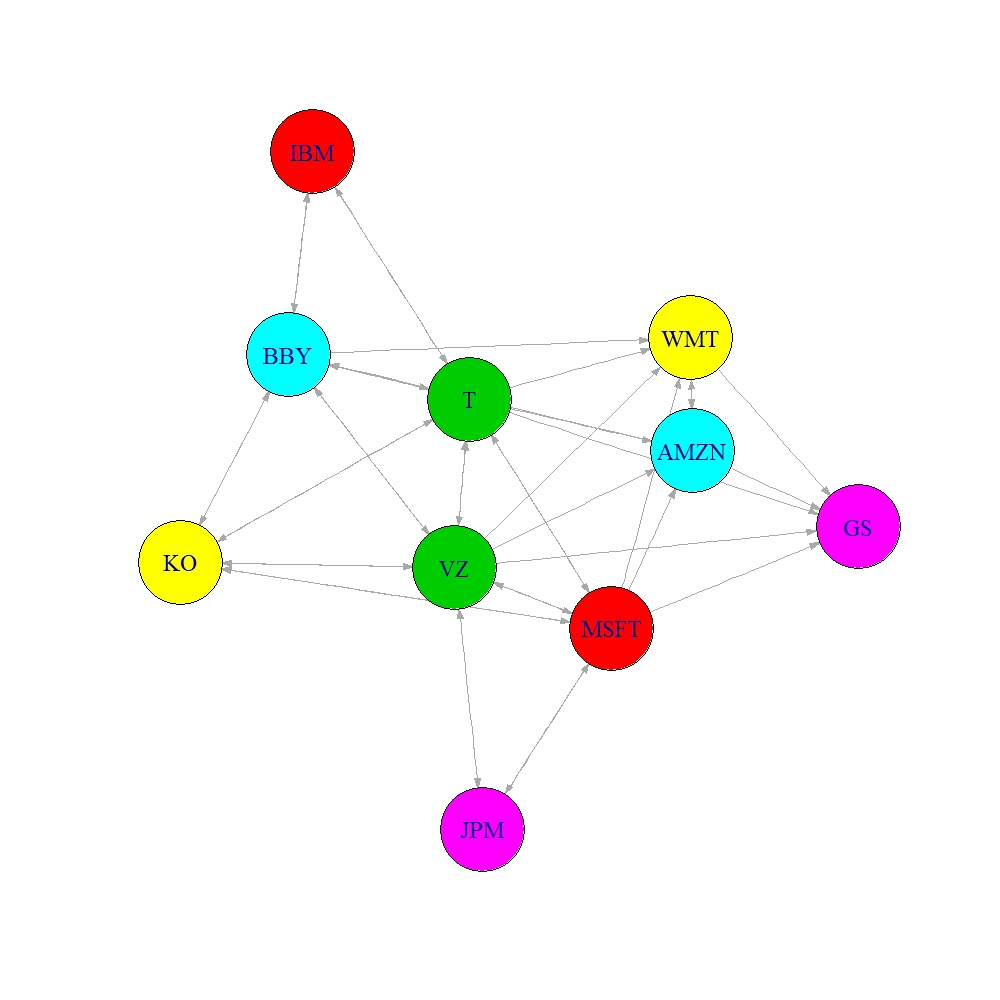
\includegraphics[width=.25\textwidth]{10stocks.jpeg}
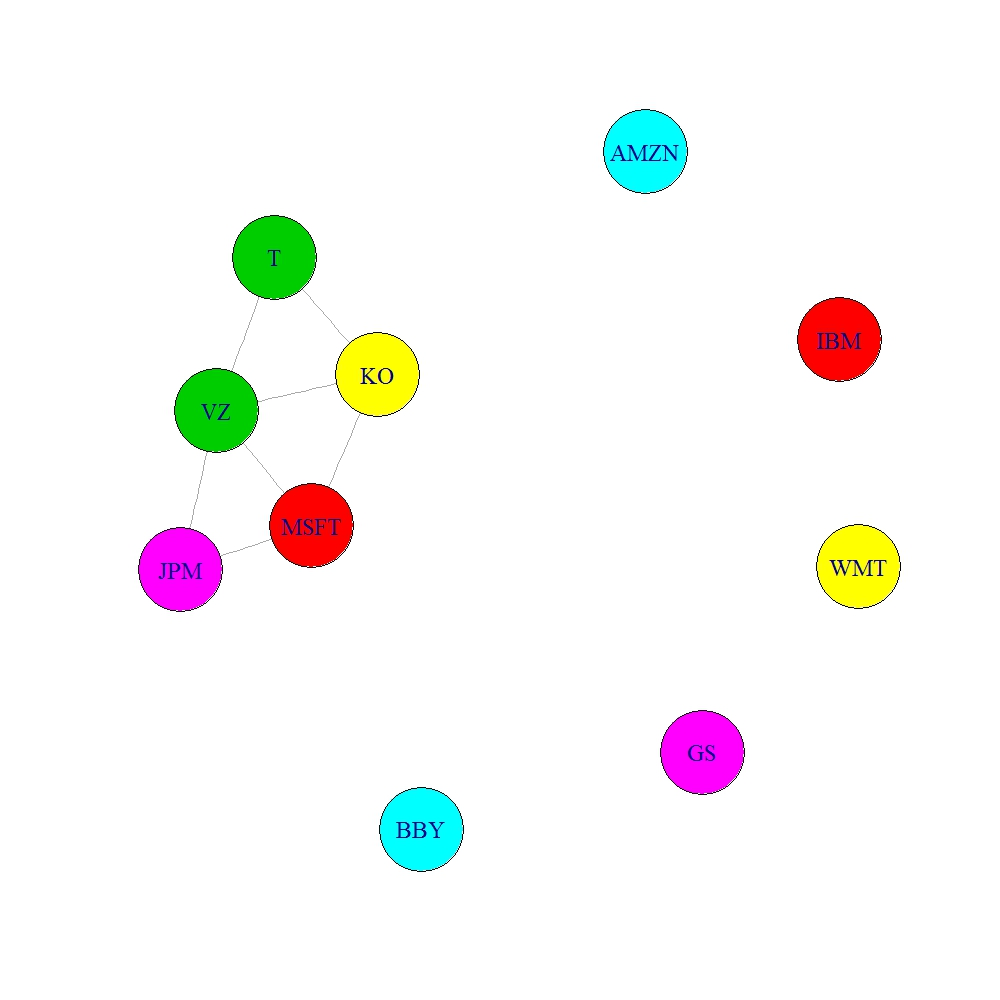
\includegraphics[width=.25\textwidth]{10stocks_huge.jpeg}
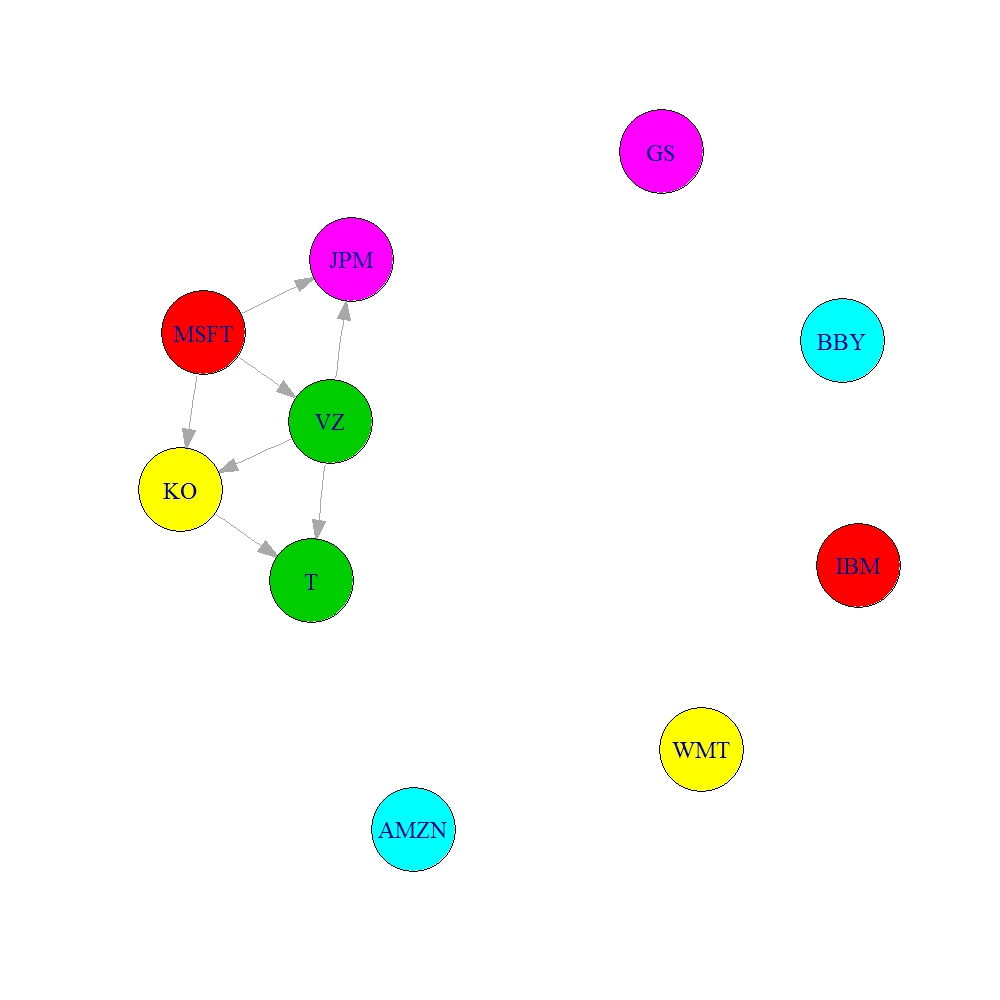
\includegraphics[width=.25\textwidth]{10stocks_bn_glasso.jpeg}
\caption{Bayesian network structures for 10 stock companies} \label{fig.8.}
\end{figure}

Results for total stocks:\\
\begin{figure}[H]\centering
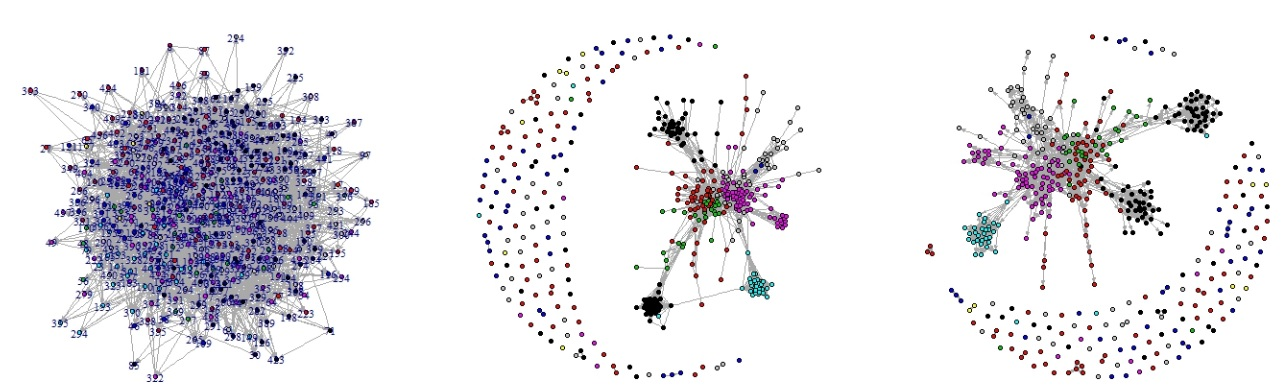
\includegraphics[width=0.8\textwidth]{stock.jpg}
\caption{Bayesian network structures for total stock companies} \label{fig.9.}

\end{figure}

CPU Time:\\
We changed the number of samples from 50 to 800, doubled each time to test the running time for the different machine learning methods:\\
For R:\\
\begin{figure}[H]\centering
     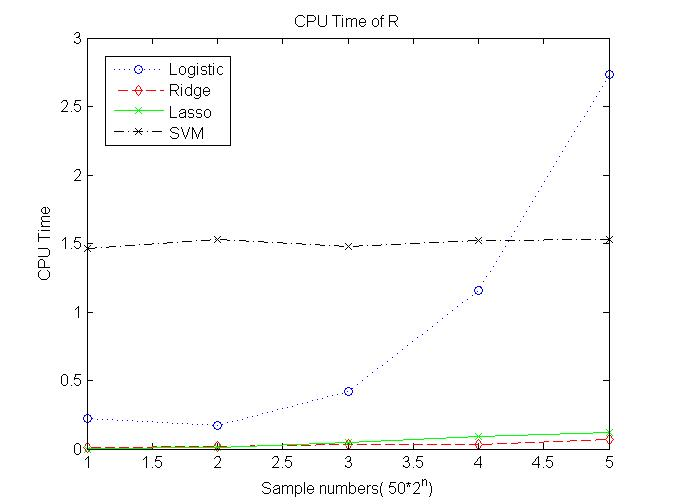
\includegraphics[width=0.5\textwidth, height=0.3\textheight]{cputime_r.jpg}
     \caption{CPU time for R} \label{fig.10.}

    \end{figure}
For Python:\\
\begin{figure}[H]\centering
     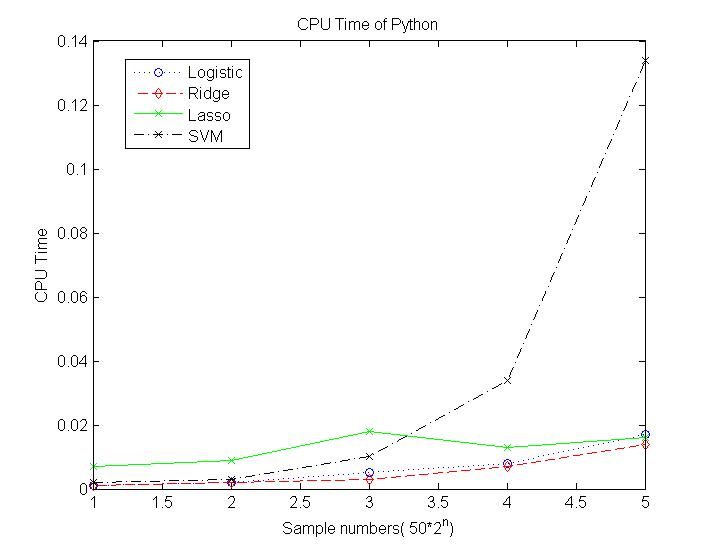
\includegraphics[width=0.5\textwidth, height=0.3\textheight]{cputime_python.jpg}
     \caption{CPU time for python} \label{fig.11.}

    \end{figure}
For R and Python:\\
  \begin{figure}[H]\centering
     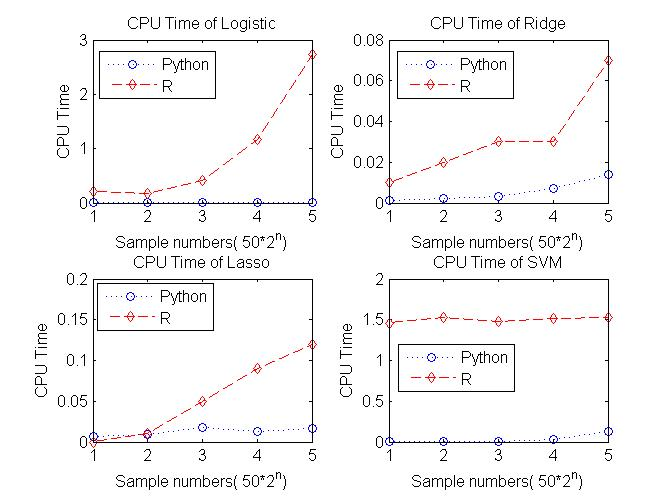
\includegraphics[width=0.7\textwidth, height=0.4\textheight]{cputime_python_r.jpg}
     \caption{CPU time for R and python} \label{fig.12.}

    \end{figure}

Accuracy rate:\\
\begin{table}[h!]\large
  \caption{Accuracy rate}
\begin{center}
    \begin{tabular}{| c | c| c | }
    \hline
    Methods& Python &  R\\
    \hline
Logistic  &77.8\%&	65.4\%\\
Ridge($\lambda$=1)&73.9\%	&77.4\%\\
Lasso($\lambda$=0.01)&78.6\%&	79.0\%\\
svm(linear)&72.4\%	&65.8\%\\
svm(poly)&74.3\%&	65.0\%\\
svm(rbf)&75.1\%	&72.8\%\\
\hline
\end{tabular}
\end{center}
\end{table}

\textbf{2.Prediction analysis}\\

\begin{equation}
R_t^{GS} = \sum_{i=1:5}{\sum_{j=1:454}\beta_{i,j}R_{t-i}^j}
\end{equation}

\begin{table}[h!]\large
  \caption{Accuracy rate and CPU time}
\begin{center}
    \begin{tabular}{| c | c|c|}
    \hline
    Methods& Accuracy rate& CPU time \\
    \hline
Logistic  &51.2\%&0.1210\\
Ridge($\lambda$=1)&54.0\%&0.1230\\
Lasso($\lambda$=0.01)&49.2\%&0.0940\\
svm(linear)&52.8\%&1.1931\\
svm(poly)&45.6\%&1.2800	\\
svm(rbf)&47.2\%&1.2921\\
\hline
\end{tabular}
\end{center}
\end{table}

\section{[Future work]}

 \begin{itemize}
        \item  Compare with the time series model, such as Garch
        \item  Deal with the high frequency data instead of daily data
\end{itemize}

\end{homeworkProblem}
\end{document} 